\documentclass[journal=jacsat,manuscript=article]{achemso}

\usepackage[version=3]{mhchem} % Formula subscripts using \ce{}
\usepackage[T1]{fontenc}       % Use modern font encodings
\usepackage{siunitx}
\DeclareSIUnit\Molar{\textsc{m}}
% !TeX root = ./azurin.tex
\usepackage{xr}
\externaldocument{Sup_info}
\newcommand*\mycommand[1]{\texttt{\emph{#1}}}

\author{Authors}
\affiliation{Huygens-Kamerlingh Onnes Laboratory, Leiden University, RA, Leiden, The Netherlands}
\email{corresponding_author@physics.leidenuniv.nl}
\title[]
{A single azurin reveals intermolecular, intramolecular electron transfer and dynamic rates.}

\abbreviations{FCS}
\keywords{American Chemical Society, \LaTeX}

\begin{document}
%%%%%%%%%%%%%%%%%%%%%%%%%%%%%%%%%%%%%%%%%%%%%%%%%%%%%%%%%%%%%%%%%%
%%%%%%% Start the main part of the manuscript here.%%%%%%%%%%%%%%
%%%%%%%%%%%%%%%%%%%%%%%%%%%%%%%%%%%%%%%%%%%%%%%%%%%%%%%%%%%%%%%%%%
\section{Introduction}
Introduction here.
\section{Experimental Section}
\subsection{Protein synthesis}
Azurin (wild type) from Pseudomona aeruginosa was expressed in E. Coli and purified as described before \citep{kamp1990purification}. BL21 E.coli was transformed with PGK22 plasmid that has gene for azurin expression. The cells were cultured in luria broth (LB) medium. Then the cells were harvested and resuspended in 20 \% (w/v) sucrose solution in Tris pH 8 buffer containing 1 mM EDTA.Then the solution was centrifuged at 8000 rpm and the supernatant was collected. Copper sulfate was added to the solution for insertion into the active site of azurin. The unwanted proteins were precipitated by addition of acetic acid until pH 4. Again the turbid solution was centrifuged to separate azurin that remained in the supernatant. The azurin solution was loaded on a CM Sepharose fast flow column and elution was performed in an Akta purifier (GE Healthcare) with a pH gradient from 4 to 6.9 in 50 mM ammonium acetate. Fractions containing azurin collected and reduced with sodium dithionite. At this moment the solution both zinc and copper azurin. The azurins were putified in a DEAE sepharose column by a salt gradient of 0 to 50 mM NaCl in Tris pH8 buffer. Fractions containing copper azurin and zinc azurin collected and concentrated separately. The purity of the samples were checked by sodium dodecyl sulphate (SDS)-polyacrylamide gel electrophoresis (PAGE) and UV/Vis spectroscopy (Cary 50 spectrophotometer, Varian Inc., Agilent Technologies, USA). The azurins appeared on SDS gel page at \~14 kDa. Both zinc and copper azurin showed a characteristic peak at \~290 nm while Cu azurin showed an additional broad absorption peak at $620 nm$ as can be seen in figure S\ref{SIfig: switching} when oxidized. The ratio $O.D_{628 nm}/O.D_{280}$ for Cu azurin was 0.56 which indcated that all the azurin molecules had a Cu atom. The concentrated protein was stored at $-80^0 C$ until further use.
\subsection{Fluorescent labeling}
The labeling protocol was based on the previous work \cite{nicolardi2012topdown}. ATTO 655 NHS-ester was bought from ATTO-TEC GmbH. The buffer containing azurin was replaced with HEPES pH 8.3 and all the amine containg impurities were removed. A mixture of 200 $\mu$M azurin and ATTO 655 NHS-ester (ration 1:1) was incubated for 45 min. The NHS-ester group reacts to one of the amine group on the protein. The unreacted dyes were removed by a HiTrap desalting column. The labeled protein was concentrated in Tris pH 8.5 buffer by centrifusing in a 3 kDa Amicon ultra filter. The labeled protein further purified by an ion exchange chromatography in a 1 mL MonoQ column (GE Health). The different peaks obtained (see figure S\ref{SIfig: peak_sep}) corresponds to the different number and position of the dye on azurin. The peak-III corresponds to the protein labeled at Lysine122 position \cite{nicolardi2012topdown}. For this position of the dye, the protein construct shows high fluorescence switching (90 \%) ratio between oxidized and reduced condition as can be seen in Figure S\ref{SIfig: peak_sep}. This fraction was choosen for our single-molecule experiemnt as the two states can be observed easily. The same protocol was used for Zn azurin labeling and similar peak separation observed. The fluorescent labeled protein was then reacted with biotin-peg-NHS (MW 3400) in PBS pH 7.4 buffer with a ratio 1:5 to make sure each protein has at least one biotin. The free biotin was then remove centrifusing in a 3kDa Amicon ultra filter. The biotin on the protein will be used for immobilization on glass surface.
\subsection{Functionalization fo coverslip}
Glass coverslips (Menzel-Glaser, 22mm × 40 mm, no. 1 thickness) were used for immobilization.The coverslips were sonicated in water (15 min) and acetone(15 min). Then they were rinsed in Milli-Q water several timesand incubated in a H2O/NH4OH/H2O2(5:1:1) bath at \SI{70}{\celsius}. The coverslips were rinsed several times with water and ethanol and finally stored in ethanol. Before functionalization, the slides were flamed. Then they were treated for 30 min with a 1\% solution of [3-(2-aminoethyl)aminopropyl]trimethoxysilane in methanol containing 5\% glacial acetic acid. This results in the binding of the active hydroxyl groups. The silane is not yet covalently bound. This is obtained by baking the coverslips in an oven at \SI{65}{\celsius} for 3 hours. After this treatment, the cover slips were sonicated for 10 minutes and washed with methanol. Dried with clean nitrogen, they were left in a desiccator overnight. The next day they were treated with a mixture of 5 mg/mL methoxy-peg-N-hydroxysuccinimide (MW 2000, Laysan Bio) and 0.05 mg/mL
biotin-peg-N-hydroxysuccinimide (MW 3400, Laysan Bio) in 50 mM phosphate buffered saline (PBS) with pH 7.4. This creates a surface containing biotin and methoxy end groups. The biotin then will bind to the NeutrAvidin with the CuAz attached to it (next section). The slides were dried with gentle flow of nitrogen and stored in a desiccator until further use.
\subsection{Protein immobilization}
The functionalized glass slide was incubated with 20 mM PBS pH 7.4 buffer for 5 min. 100 nM of Neutravidin (Thermo Scientific) was incubated for another 15 min and then washed to remove unbound Neutravidin. 100 pM of the labeled protein was then incubated for 1 min to get isolated proteins (20 per \SI{100}{\micro\meter} area) on the functionalized glass surface. The unbound proteins were then removed by replacing with a fresh PBS buffer.
\subsection{Electrochemical-poteontial control}
Once the unbound proteins are removed, a new mixture containing 0.1 mM sodium ascorbate ($[C_6H_7O_6]^-Na^+$) and 0.2 mM potassium ferricyanide ($[Fe(CN)_6]^{3-}$) in 4 mL PBS pH 7.4 was added at the sample holder which were our initial oxidant and reductant. Electrochemical potential of the solution is obtained from the ratio of oxidant and reductant. The ratio of of oxidant and redcuctant were further controled by a potentiostat (Model 800B Series Electrochemical Detector, CH Instruments). A platinum rectangular grid (the total length/ width of the grid is around 2.5 cm) was used as working electrode and pressed onto the sample slide with the help of a small glass slide. Not only is the pressure evenly applied on the grid, but also small confined volumes are formed where the sample slide and glass slide form the ’floor’ and ’roof’ and the platinum grid forms the ’walls’. A part of the platinum grid was exposed to the solution. These confined volumes are in the order of nanoliters, which makes switching of elctrochemical potential of solution possible in a matter of minutes.

%%%%%%Results and Discussion%%%%%%%%%
\section{Results and discussion\label{sec:results}}
%Scheme
\begin{scheme}
	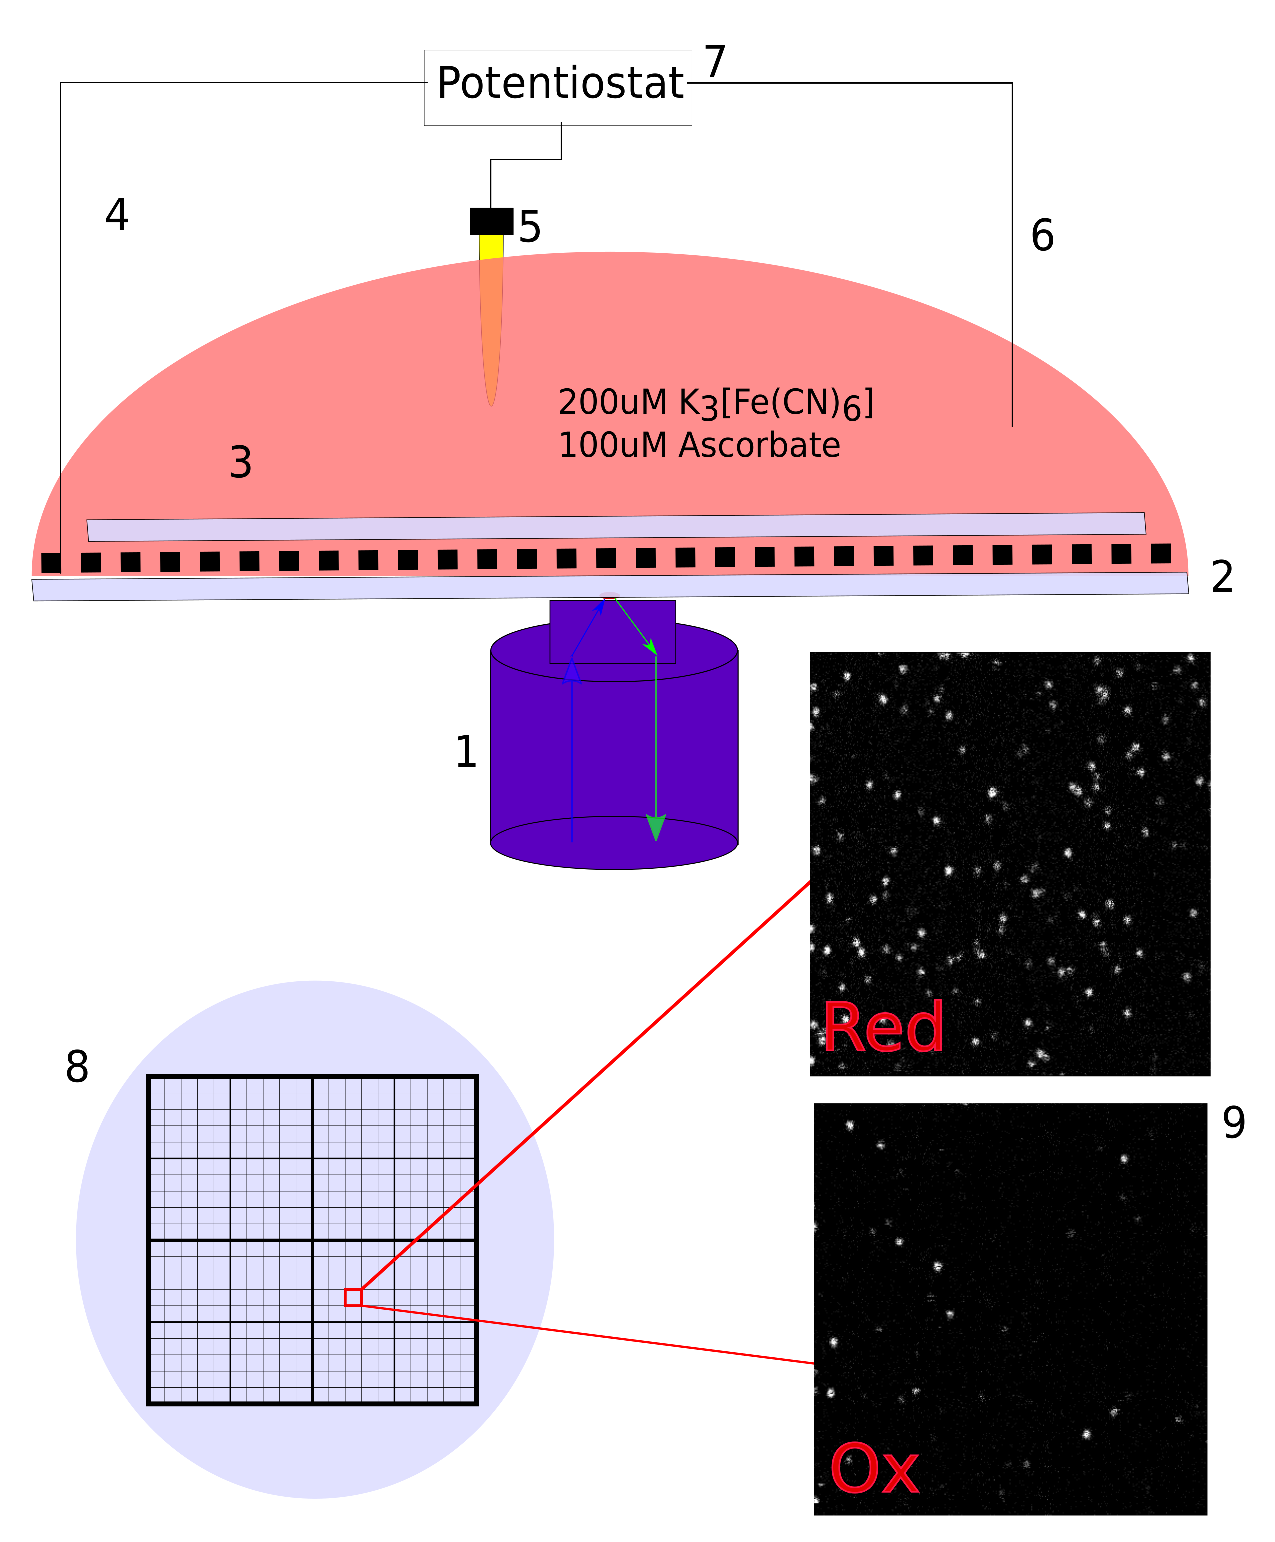
\includegraphics[scale=0.8]{Figure/Scheme_1_setup.eps}
	\caption{The scheme picture of the final setup. \textbf{(1)}  Objective through which light is irradiated on and collected from the sample. \textbf{(2)} The functionalized sample slide with on top the platinum grid
	and another small glass slide to press the grid on the sample slide, resulting in small confined volumes in the order of nanoliters. \textbf{(3)} The electron mediator solution consisting of \SI{200}{\micro\Molar} ferricyanide, \SI{100}{\micro\Molar} ascorbate in PBS (PH 7.4) buffer with a total volume of 4 mL. \textbf{(4)} The working electrode (Platinum wire) that is in contact with the platinum grid. \textbf{(5)} The saturated calomel reference electrode. \textbf{(6)} The Platinum wire (not touching the grid) as counter electrode. \textbf{(7)} The potentiostat (Model 800B Series Electrochemical Detector, CH Instruments) to which the electrodes are connected. \textbf{(8)}, \textbf{(9)} Top view of the sample slide and two images are showing the labeled Cu-Azurin reduced(brighter) and oxidized(dimmer).}
  	\label{sch:setup}
\end{scheme}
%time trace
\begin{figure}
	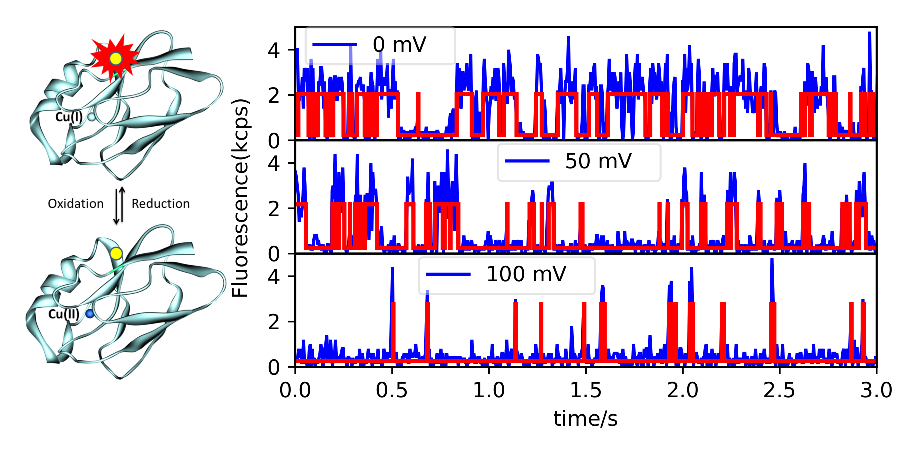
\includegraphics[width=\textwidth]{Figure/Figure_1_timetrace_CuAzu.eps}
	\caption{Time traces of Cu-Azurin labeled with ATTO655 at different potentials. The structure of the protein with properly positioned dye can be seen in the schematic picture in the left. In Cu(II) state (shown in bluish atom in the protein structure), the dye is non fluorescent because of FRET and in Cu(I) state (shown in gray atom), the dye is fluorescent. Notice the amount of time the protein spends on bright and dark state at different potentials. At lower potentials (e.g 0 mV) the protein is brighter most of the time because of the higher concentration of reductant.}
	\label{fig:timetrace}
\end{figure}
%Midpoint histogram
\begin{figure}
	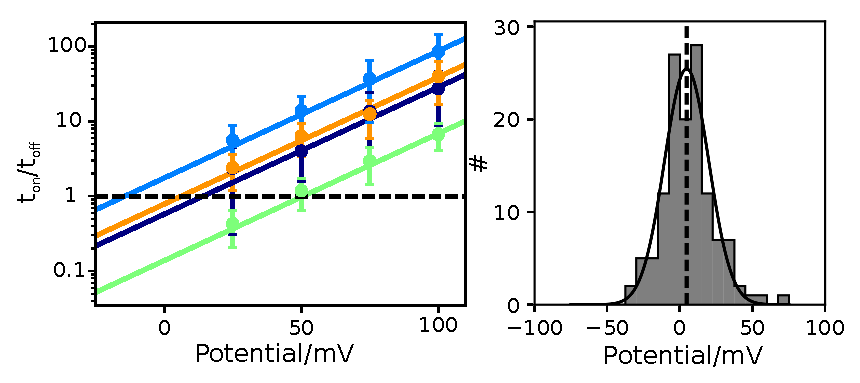
\includegraphics[width=\textwidth]{Figure/Figure_2_midpoint.eps}
	\caption{Ratio between on and off time as a function of applied potential for the same single-molecule. Different color represents different single-molecules. And the line connecting the data points is the Nernst fit for all the data points above 25 mV. The plot in the right is the histogram of midpoint potentials for $132$ molecules with a gaussian fit with center 4.5 mV with respect to calomel electrode.}
	\label{fig:midpoint}
\end{figure}
%on-off 1D histogram
\begin{figure}
	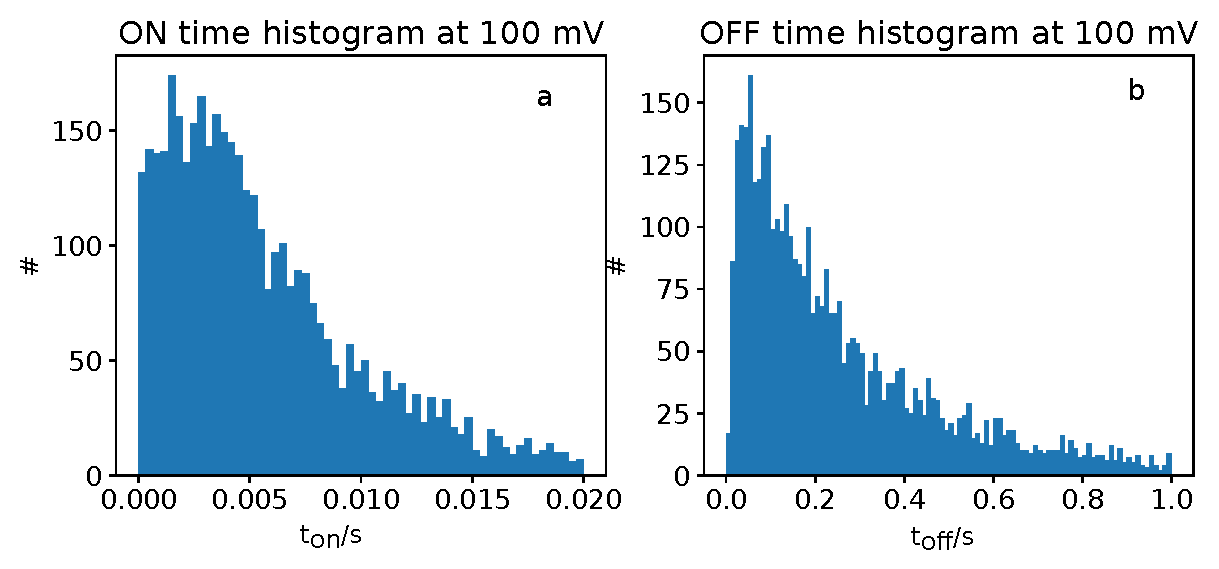
\includegraphics[width=\textwidth]{Figure/Figure_3_on_off_1D.eps}
	\caption{\textbf{On off histogram.} The histogram of on-times(a) and of off-times(b) of Cu-Azurin-ATTO655 showing rise time. This indicates that both oxidation and reduction of Cu-Azurin occurs through an intermediate step.}
	\label{fig:onoff1D}
\end{figure}
%Dynamic rates. protein showing diiferent rates with time
\begin{figure}
	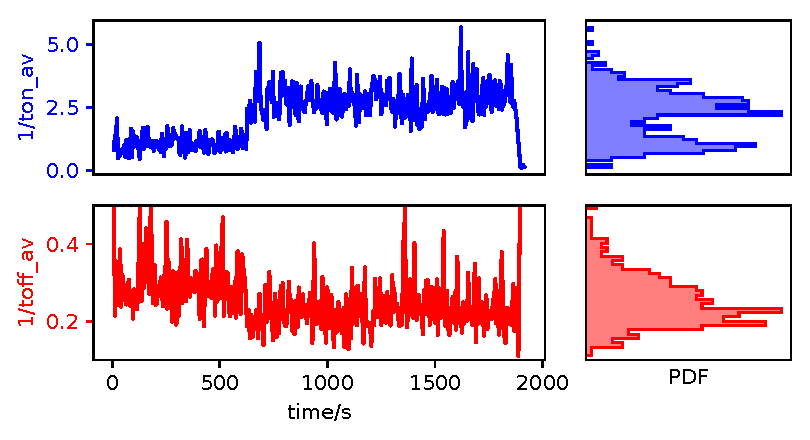
\includegraphics[width=\textwidth]{Figure/dynamic_rates.eps}
	\caption{\textbf{Dynamics in the turnovers of the protein.}}
	\label{fig:dynamic_rates}
\end{figure}
%on-off 2D histogram
\begin{figure}
	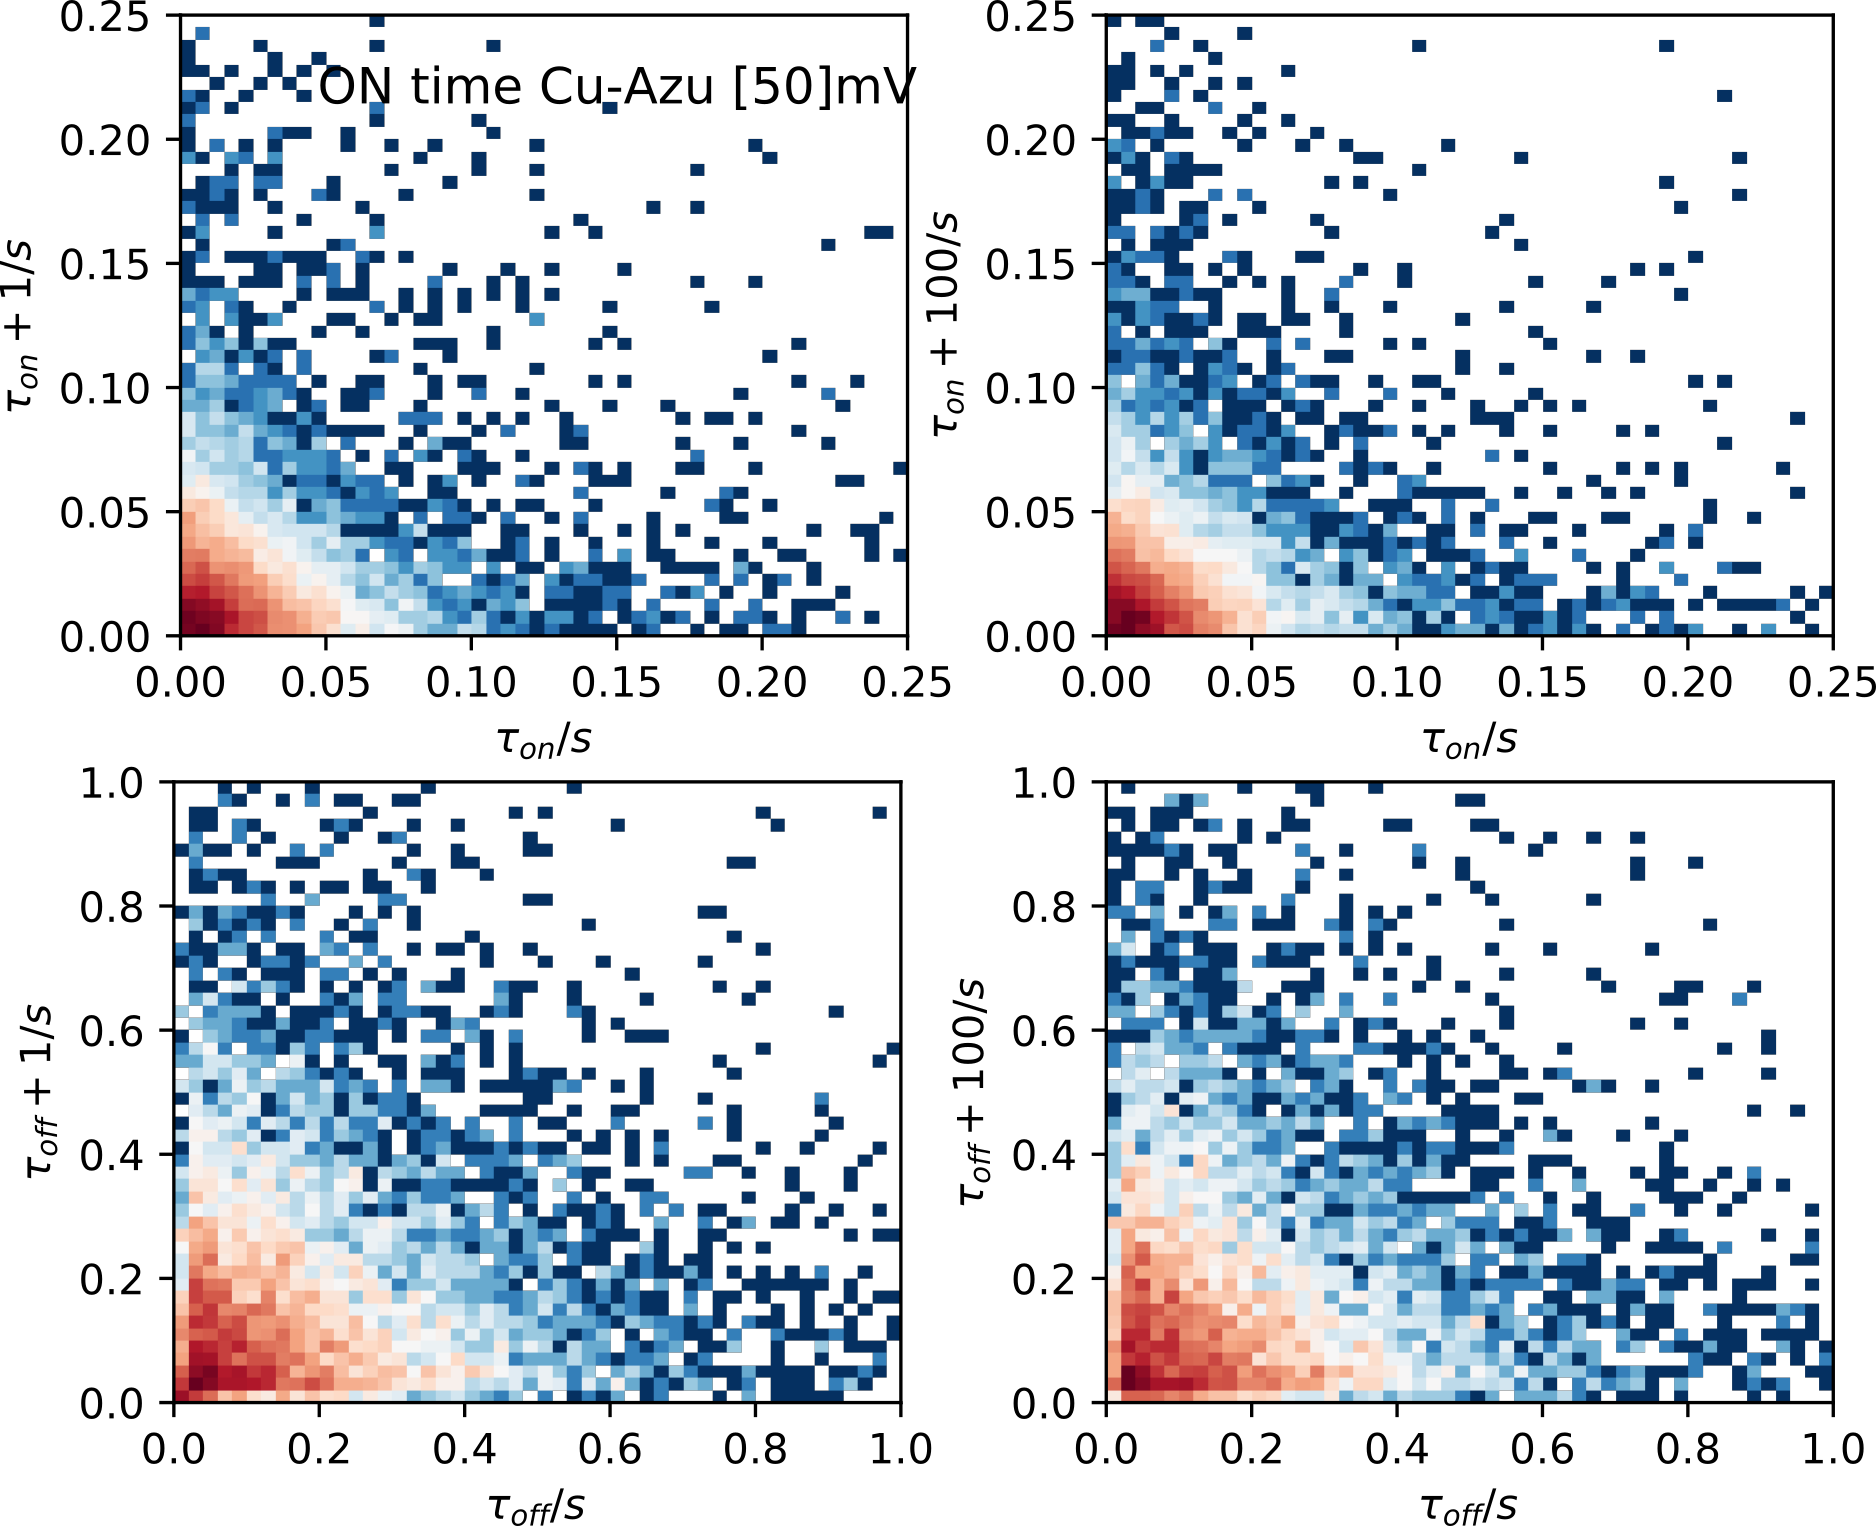
\includegraphics[width=\textwidth]{Figure/Figure_4_on_off_2D_100mV.png}
	\caption{\textbf{2D histogram: Cu-Azurin.} 2D correlation plot of (a) on-times vs the next on-times (b) on-times vs the on-time after 100 turnovers (c) off-times vs next off-times (d) off-times vs the off-time after 100 turnovers.}
	\label{fig:onoff2D}
\end{figure}

%Intramolecular electron transfer reaction
\begin{figure}
	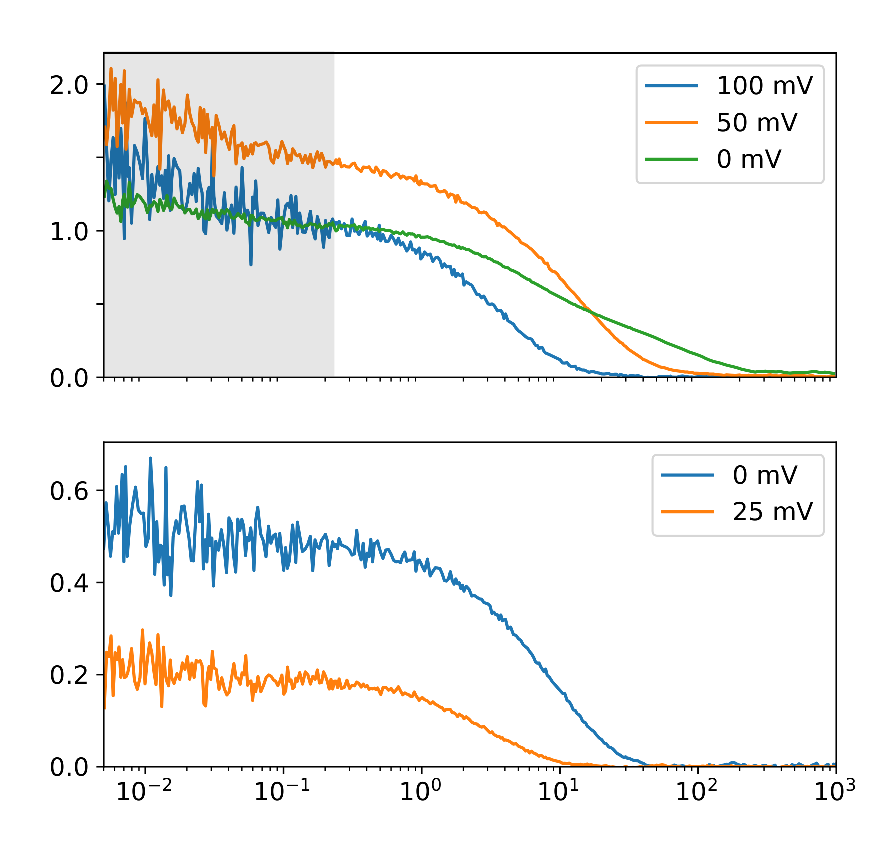
\includegraphics[width=\textwidth]{Figure/fcs_components.eps}
	\caption{\textbf{Intramolecular electron transfer.} Shorter decay with time constant fo around 30 us}
	\label{fig:fcs_components}
\end{figure}
%%%%%Experimental Section%%%%%%%%%%
\section%{Experimental}
%%%%\bibliographystyle{achemso.bst}
\bibliography{azurin}
\end{document}